\documentclass[10pt]{article}
\usepackage{pset}
\usepackage{multicol,graphicx}

\begin{document}


\nobibliography*

\title{Programming Assignment 2: Scaling with SGD}
\author{CS4787 --- Principles of Large-Scale Machine Learning Systems}
\date{}

\maketitle
%\begin{multicols}{2}

\textbf{Part I: Summary}
In this assignment, I was able to implement the four versions of Stochastic Gradient Descent with fixed step size $\alpha$ from the write-up: Regular SGD, Sequential SGD, and two forms of SGD with mini-batching, namely Mini-batch SGD and Sequential Mini-batch SGD. 

The four algorithms performed very decently throughout the first 10 epochs of training, with the training and test error going down almost asymptotically to a little over .08\% and just about 0.08\%, respectively. Nonetheless, the runtime varied greatly among the four algorithms, with the sequential versions of regular and mini-batch SGD being faster their respective, randomly sampled counterparts.

The four algorithms are very close in terms of accuracy, and thus we are not able to call any of them a clear winner, but as mentioned above, in terms of runtime, sequential mini-batch SGD performs the best. For $\alpha = 0.001$ with Algorithms 1 and 2, and $\alpha_m = 0.05$ for Algorithms 3 and 4 , all four algorithms bring the training and test error down at a pretty similar rate as a function of epochs. It is important to note, however, that the different step sizes are actually two orders of magnitude apart - but SGD and Sequential SGD make many more updates per epoch than their mini-batch counterparts, hence the smaller value of $\alpha$ produces a similar decrease in the error rates. It is important to note that the error does change a lot depending on the value of $\alpha$, and even more over different batch sizes, nonetheless, and so these must be chosen wisely to make good use of any of these algorithms.

Below are the plots for training and test error for all four algorithms using the parameters specified in the write-up. In addition, I list the optimal parameters found for the respective exploration sections in a table below.
\begin{center}
\begin{tabular}{|c|c|} \hline
     Section & Parameters \\ \hline
     2.2 & $\alpha = 0.00348$ \\
     2.3 & $\alpha = 0.00348$ \\
     2.4 & $\alpha = 0.057$ and $B = 16$\\ \hline
\end{tabular}
\end{center}
\begin{center}
    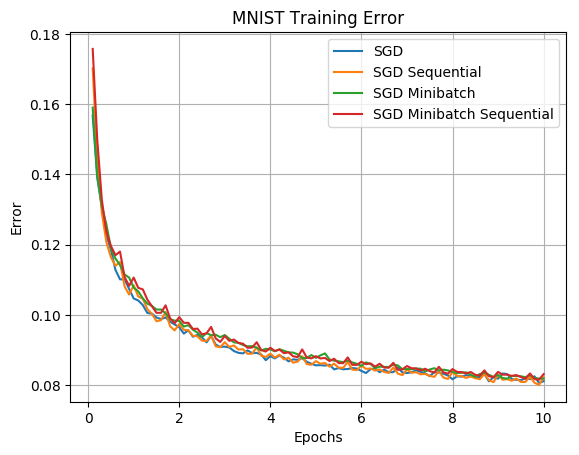
\includegraphics[width=.45\textwidth]{training.png}
    \label{fig:tr_er}
\end{center}
\begin{center}
    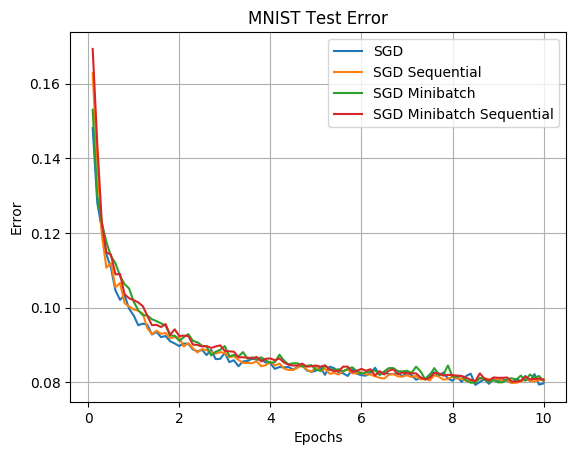
\includegraphics[width=.45\textwidth]{test.png}
    \label{fig:te_er}
\end{center}


\textbf{Part II: Exploration}
For the first part of the exploration, I evaluated the algorithms training and test error after ten epochs of training with $\alpha = .0002$. The plots are shown below, and clearly, the algorithm does not perform as well: the steps were probably too short to make as much progress as we did with a larger step size over the same number of iterations (although if we had ran the algorithm for longer, we might have obtained a better test error).

\begin{center}
    \includegraphics[width=.45\textwidth]{SGDExplorationTraining.png}
    %\caption{Training error of the model as a function of epochs for $\alpha = 2e-4$. The minimum error obtained is larger than with $\alpha=1e-3.$}
    \label{fig:ex_p1tr}
\end{center}
\begin{center}
    \includegraphics[width=.45\textwidth]{SGDExplorationTest.png}
    \label{fig:ex_p1te}
\end{center}

To obtain a value of $\alpha$ with which to obtain, within 5 epochs, a training error comparable to the training error obtained by running 10 epochs of SGD with the parameters specified in the assignment write-up, I implemented grid search around various neighborhoods of $\mathbb{R}^+$. I then identified the model with the lowest average error over the last three model updates, and plotted the training and test error below. The training error is able to go down as much as 0.078\%, but the test error seems to plateau at around .08\% (also, ignore the 10 in the title in the plots below - its supposed to be a 5).

Below, we also list some of the values of $\alpha$ used in this part of the exploration, where $start:end:step$ takes the obvious meaning:

$$ \{\alpha\} = \{.003:0.0035:.00001\} \cup \{0.001:0.0015:0.0001\} \cup \{ 0.002:0.0024:0.0002\} \cup ...$$

\begin{center}
    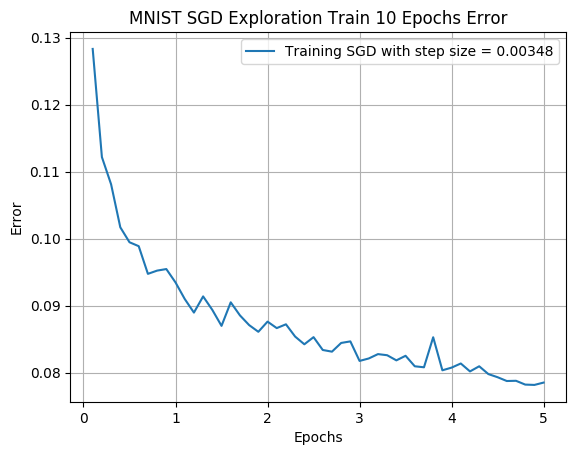
\includegraphics[width=.45\textwidth]{SGDExplorationTrain5Epochs.png}
    \label{fig:expl3tr}
\end{center}

\begin{center}
    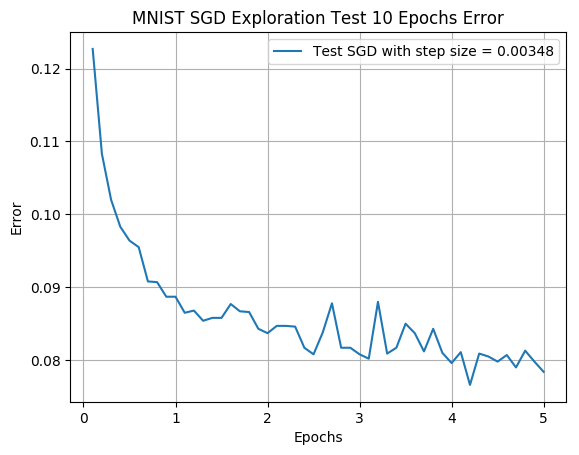
\includegraphics[width=.45\textwidth]{SGDExplorationTest5Epochs.png}
    \label{fig:expl3te}
\end{center}

Of course, this value of $\alpha$ also allows us to get a lower training error after 10 epochs, so we show the plots for the training and test error over 10 epochs (for a different run) below. Interestingly, the test error also went down almost monotonously although a bit more slowly - so we are not overfitting yet.

\begin{center}
    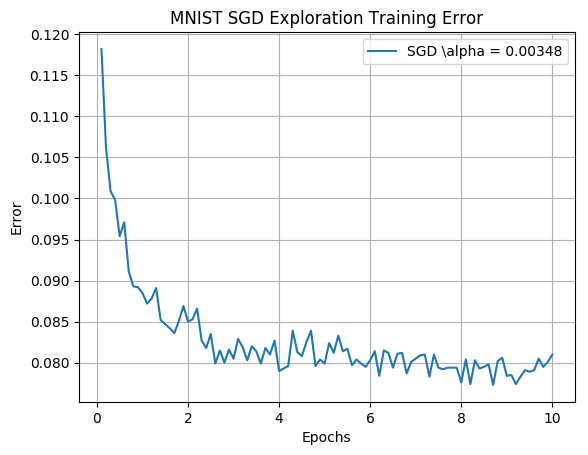
\includegraphics[width=.45\textwidth]{SGDExplorationTraining10.png}
    \label{fig:expl2tr}
\end{center}
\begin{center}
    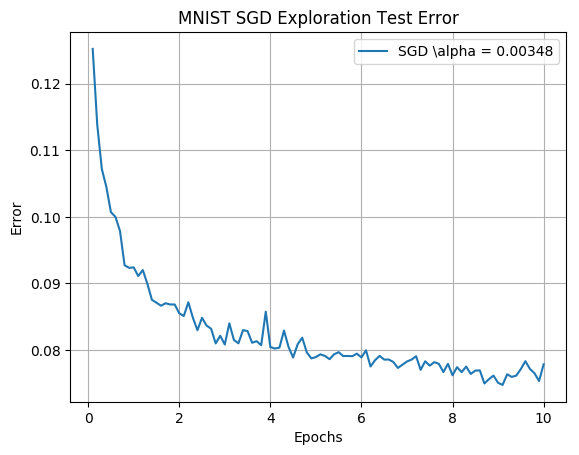
\includegraphics[width=.45\textwidth]{SGDExplorationTest10.png}
    \label{fig:expl2te}
\end{center}

Lastly, to find values of $\alpha$ and batch size $B$ with which we could attain, after five epochs, a training error that is comparable to the one we obtained by running 10 epochs of SGD with Sequential Mini-batching using the parameters specified in the assignment write-up, I used naive grid search and recorded the average training error of the last few model updates saved. Each time I performed this search over a different domain, I found the model with the least training error (computed over the last three updates), and plotted its training and test error. The plots can be seen below.

Of course, I could have also used $B=1$ and $\alpha = 0.00348$ as in the previous exploration part to get a lower training error, since the training error of mini-batch sequential SGD was also about 0.08\% and these parameters allow for the algorithm to decrease the training error even further.

\begin{center}
    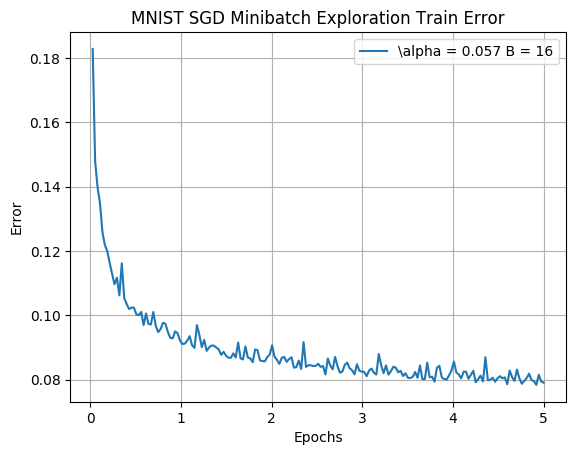
\includegraphics[width=.45\textwidth]{SGDMinibatchExplorationTrain_final.png}
    \label{fig:expl4tr}
\end{center}
\begin{center}
    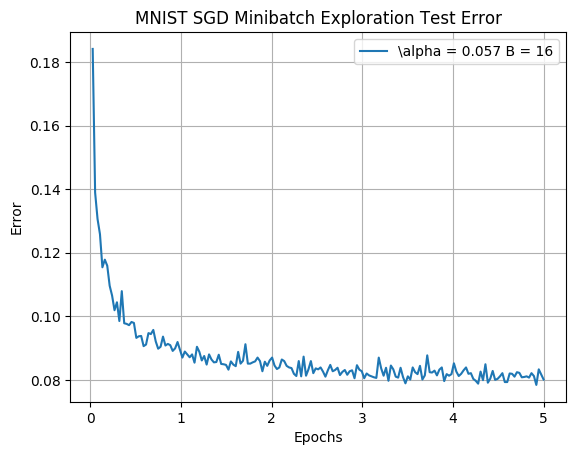
\includegraphics[width=.45\textwidth]{SGDMinibatchExplorationTest_final.png}
    \label{fig:expl4te}
\end{center}


\textbf{Part III: Systems Evaluation} \\
There is a clear winner from these four algorithms in terms of runtime, as can be seen in the following bar graph:
\begin{center}
    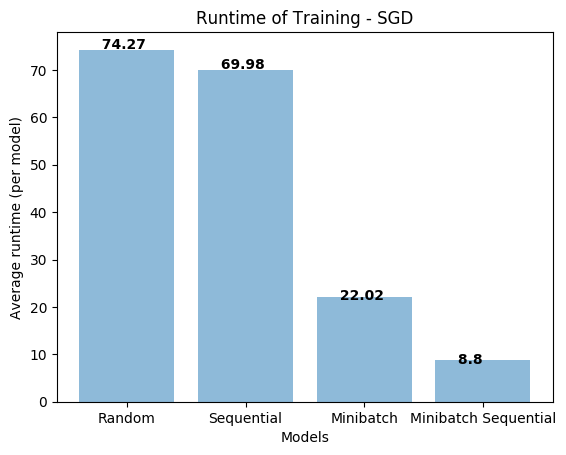
\includegraphics[width=.45\textwidth]{train_time.png}
    \label{fig:tr_ti}
\end{center}
Regular SGD with random sampling takes the most time, averaging 74.27 seconds for all 10 epochs, over five trials. Sequential SGD is a close second-to-last, averaging 69.98 seconds over five trials. As mentioned in the project description, this is due to poor memory locality of Algorithm 1 as the hardware is not able to predict with any reasonable accuracy what the next data point to be fetched is, while for Algorithm 2 the hardware has a better chance at doing this.

By making use of parallelization, mini-batching by itself is able to improve the runtime from Algorithms 1 and 2 with an average runtime of 22.02 seconds over five trials; but again, choosing a mini-batch uniformly at random (and with replacement) from our training set has poor memory locality, so SGD with Sequential Mini-batching is clearly faster, and by far the fastest algorithm, averaging 8.8 seconds per 10 epochs, over five trials.
%\end{multicols}
\end{document}
